\documentclass[11pt, final, journal, a4paper]{IEEEtran}

\usepackage[dutch]{babel}
\usepackage[utf8]{inputenc}
\usepackage{natbib}
\usepackage{subfigure}
\usepackage{tikz,pgfplots}

\title{Onderzoek naar Blackjack-strategieën \\ {\large Groep 20}}
\author{\IEEEauthorblockN{Jan {Van Braeckel},}
\and
\IEEEauthorblockN{Annemie {De Groote},}
\and
\IEEEauthorblockN{Lara {Delange},}
\and
\IEEEauthorblockN{Jasper {De Vrient}}}
\date{\today}

\begin{document}
\maketitle

\begin{abstract}
Als u naar goede strategieën zoekt om Blackjack te winnen, vindt u op het internet snel tabellen met verscheidene waarden in. Deze tabellen geven een indicatie over wanneer u uw hand het best weggooit of wanneer u een kaart bij moet vragen. Het is natuurlijk handig, maar wanneer is het nu het best om te standen of te splitten?
\end{abstract}

\section{Inleiding}
Als semesteropdracht voor het vak Onderzoekstechnieken kregen wij de opdracht het spelletje Blackjack te analyseren. Dit met het doel om na te gaan of er een strategie kan bedacht worden om het gokspel zo veel mogelijk te winnen. Volgens de casino's bestaat er geen ideale strategie, wel wordt er al tientallen jaren onderzoek naar gevoerd. We ontdekten dat er zowel onderzoeken van wiskundigen als van ervaren spelers bestaan. Het doel van dit artikel is om te bekijken wanneer een speler de beste waarde heeft om te standen of om te splitten.

\section{Onderzoeksvragen}
Aangezien er verschillende strategieën bestaan en iedere strategie een eigen focus heeft, kiezen we ervoor ons toe te spitsen op het splitten en standen van een hand. Tijdens ons literair onderzoek ontdekten we dat deze twee termen vaak een rol spelen in de verschillende, bestaande strategieën, waardoor de nieuwsgierigheid groeide om dit te onderzoeken. 
De eerste onderzoeksvraag gaat dieper in op het beste cijfer om te standen. Dit betekent dat de speler daarna geen kaarten meer bij vraagt. We weten dat de dealer altijd stopt bij kaarten gelijk of hoger aan zeventien, geldt hetzelfde voor de speler? De tweede vraag onderzoekt wanneer men het best kan splitten.
\\\\
Hieronder worden de vragen kort vermeld:
\begin{itemize}
	\item Welke totaalwaarde van de hand is het beste om te standen?
	\item Welk koppel van waarden is het best om te splitten?
\end{itemize}

\section{Duiding literatuur}
Blackjack of `eenentwintigen' is een kaartspel waarbij één of meerdere spelers het opnemen tegen een dealer. Vroeger werd dit spel slechts met één deck, dat uit 52 kaarten bestaat,  gespeeld en werden de kaarten pas opnieuw geschud eenmaal ze allemaal gespeeld waren. Uiteraard waren er mensen die tactieken ontwikkelden om de dealer te slim af te zijn, Edward O. Thorp was zo iemand. Niet snel na de ontdekkingen van Thorp ontstonden er heel wat andere methodes. De casino's merkten na verloop van tijd dat bepaalde spelers heel veel geld wonnen. Dit fenomeen zorgde ervoor dat de set-up van Blackjack werd aangepast. Ten eerste werden er meer decks in één spel gebruikt, daarnaast werden de kaarten vaker geschud en gedeeld. Dit wordt dan de cut-off waarde genoemd.\citep{Wong1992BasicBlackjack, van1997blackjack, fogel2004evolving,Wong1993BlackJackSecrets} Daarnaast bevatten de regels veel variaties, wat betekent dat de regels van ieder casino verschillen. In dit werk bespreken we de meest gebruikte regels zoals ze in de Amerikaanse casino's te vinden zijn. In dit document hanteren we de Engelstalige terminologie. 

Bij de start van het spel krijgt elke speler twee kaarten. De eerste kaart van de dealer wordt met de waarde naar boven gelegd en de tweede kaart met de waarde naar de tafel toe. De kaarten van de speler worden standaard met de waarde naar boven gelegd. Verschillende casino’s staan het echter wel toe om de hand van de speler af te schermen. Het uiteindelijke doel van dit spel is om de dealer te verslaan zonder over 21 te gaan met de waarde van de kaarten. Indien een speler met zijn eerste twee kaarten 21 haalt, wordt dit een Blackjack genoemd. De hand van de winnaar bestaat dan uit een aas en een kaart met tien als waarde.

Een aas telt voor één of elf, naargelang hoe de speler de kaart wenst te gebruiken. De boer, koningin en koning tellen elk afzonderlijk voor tien punten. In het geval van een Blackjack stopt het spel onmiddellijk. De speler wordt uitbetaald aan een ratio van 3:2, met drie zijnde de uitbetaling en twee de inzet. Indien dealer en speler dezelfde waarde hebben bij het einde van het spel noemt men dit pushen en krijgt de speler zijn inzet terug. In de gevallen zonder Blackjack wint de speler die het dichtst bij 21 scoort. Een score van meer dan 21 betekent een direct verlies, in de casino’s wordt dit burnen genoemd. 

Zoals hierboven vermeld, heeft de aas een cruciale betekenis in het spel. Niet alleen kiest de speler de waarde van de kaart, indien de dealer na het uitdelen als open kaart een aas heeft, kan de speler `insurance' of verzekering kopen. Deze insurance kost de helft van de initiële inzet en is dus een soort van dekking. Als de dealer Blackjack heeft, krijgt de speler zijn insurance dubbel terug betaald en verliest hij niets. Als de dealer geen Blackjack heeft, verliest de speler zijn insurance.

De dealer volgt altijd een vaste strategie, hij blijft namelijk hitten (een kaart nemen) tot zijn kaartwaarde 17 of hoger is. Dit maakt het net zo interessant om te onderzoeken. Een aas wordt vaak als elf geteld, tenzij de dealer zich burnt. Bij een verbrand hand wordt de aas als een één geteld en blijft de dealer opnieuw kaarten trekken tot hij terug een waarde van 17 of hoger bezit. Aangezien de meeste dealers deze strategie hanteren, kan de speler hierop inspelen en andere strategieën benutten om de dealer te slim af te zijn. Twee van deze strategieën spelen in op `splitten' en `doublen'. 

Splitten vindt plaats als de speler na het delen twee kaarten heeft met dezelfde waarde. Indien de speler dit wenst, kan hij zijn hand splitten en met twee hands verder spelen. Wanneer dit gebeurt, moet de speler bij het tweede hand evenveel inzet plaatsen als bij zijn eerste hand. In het geval dat een speler na het splitten nog eens twee dezelfde kaarten heeft in een hand kan hij deze `resplitten'. Hierop gelden dezelfde regels als bij een gewone split.

Doublen kan de speler enkel als die twee kaarten heeft. Hier verdubbelt men de inzet en wordt er slechts één extra kaart genomen. Daarna is de dealer aan de beurt.

De hand van een speler kan `hard' of `soft' zijn. Een soft hand betekent dat de hand van de speler een aas bevat die als een 11 wordt gerekend. Ter illustratie: de speler bezit een negen en een aas. De speler beslist om een kaart bij te vragen, hierdoor burnt hij zich. De initiële waarde van de aas was een elf. Omdat de speler zich geburnt heeft, wordt de aas nu als een één gerekend. Als alle azen in de hand van de speler als een één worden geteld, spreekt men van een hard hand.

Vanzelfsprekend zal de speler zijn inzet verliezen indien de dealer een hogere kaartwaarde heeft dan de speler. Het omgekeerde is dan ook geldig: de speler wint wanneer zijn kaartwaarde hoger is dan die van de dealer.

Tijdens het doornemen van de literatuur ontdekten we verschillende cheat sheets. Dit zijn handige tabellen die de hand van de speler voorstellen. Hierdoor kan de speler beslissen wat hij het best kan doen met de verkregen kaarten \citep{Wong1992BasicBlackjack,van1997blackjack,fogel2004evolving,Wong1993BlackJackSecrets}. De manier van spelen is afhankelijk van de strategie die de dealer volgt. De cheat sheets worden zowel op het internet als in boeken en artikels aangeboden, toch rijst de vraag of deze wel correct zijn en de speler effectief een voordeel geven. Daarom onderzoeken we of de speler bij een bepaalde totaalwaarde meer kans heeft om te winnen.

De regels werden grotendeels geciteerd en vertaald uit de volgende papers: \cite{Wong1992BasicBlackjack, fogel2004evolving, van1997blackjack}.

\section{Eigen resultaten}
Het doel van dit onderzoek is om te bepalen met welk hand de speler het best split en/of stand. Om dit te kunnen bepalen, moeten we ieder hand voldoende keer tegen de dealer spelen en nadien bekijken hoeveel keer de speler en dealer gewonnen hebben. We hebben, voor het berekenen van de verschillende handen, gebruik gemaakt van bestaande software die we hebben aangepast om aan onze eisen te voldoen. De bestaande simulator ondersteunde enkel de mogelijkheid om voor een aantal seconden zoveel mogelijk hands te simuleren. Bovendien volstond de uitvoer niet aan onze verwachtingen, deze gaf enkel weer hoeveel opbrengst de speler per kaartspel had en dus niet de resultaten per hand. Daarnaast creëerden we de kans om de resultaten te exporteren.

Ten eerste werd er voorzien dat er een duidelijke invoer – simulatie – uitvoer structuur is. Het werd mogelijk gemaakt om invoerparameters te lezen van bestanden. Daarna werd er een abstractie van een simulatie gemaakt. Zo werd het mogelijk verschillende simulaties af te zonderen. Tevens werd de mogelijkheid toegevoegd om per simulatie een record op te stellen en de verkregen resultaten om te zetten naar SPSS bestanden. Deze uitvoer is per hand en niet per kaartspel.

Om de simulatie te verbeteren, werden extra elementen toegevoegd. Dit geeft de mogelijkheid om een Blackjack spel tussen speler en dealer of een ander scenario op te maken. De mogelijkheid voor het spelen van een hand volgens een bepaalde strategie was al beschikbaar, maar was niet herbruikbaar. Dit werd eveneens aangepast.

Als laatste werd er een functionaliteit aangemaakt waardoor de gebruiker simulaties kan aanbieden. Dit zorgt ervoor dat deze simulatie een bepaald aantal keren wordt uitgevoerd. U kunt de aangepaste code vinden op onze GitHub repository. 

Om te kunnen bepalen welke totaalwaarde het meest winstgevend is, hebben we ervoor gezorgd dat de omgevingsfactoren gelijk bleven. Er werd steeds met 4 decks gespeeld die een cut-off waarde van 67\% hadden. De dealer hanteerde steeds dezelfde strategie, namelijk kaarten nemen tot hij aan een waarde van 17 of hoger komt. 

Toch zijn er enkele beperkingen die we willen vermelden. Bij de simulatie houden we geen rekening met de kaarten die de speler en de dealer gekregen hebben, maar enkel met de totaalwaarde van de hand van de speler. De mogelijkheid dat de speler rekening kan houden met de kaarten die reeds uit het spel zijn, wordt dus weggenomen. Dit houdt in dat, door de simulatie, de menselijke factor is geëlimineerd en dus de rede en twijfel geen effect heeft. Deze beperkingen zorgen ervoor dat de resultaten mogelijks niet overeen komen met de werkelijkheid.

\subsection{Resultaten standen}
Om deze resultaten te bekomen, hebben we elk hand 10000 keer gesimuleerd en vervolgens gekeken wie de winnaar was. Om dit te bekomen, hebben we ervoor gezorgd dat de speler een vaste totaalwaarde had.
Volgende resultaten werden bekomen:\\
\begin{table}[h]
\centering
\caption{Winstpercentages standen}
\begin{tabular}{r||c|c||c}
																					& \multicolumn{2}{c||}{De winnaar}	&        \\ \hline
\multicolumn{1}{r||}{Speler stopt op}   	& Dealer         & Speler         	& Totaal \\ \hline \hline
\multicolumn{1}{r||}2  										& 74\%           & 26\%           	& 100\%  \\ \hline
\multicolumn{1}{r||}3  										& 74\%           & 26\%           	& 100\%  \\ \hline
\multicolumn{1}{r||}4  										& 74\%           & 26\%           	& 100\%  \\ \hline
\multicolumn{1}{r||}5  										& 74\%           & 26\%           	& 100\%  \\ \hline
\multicolumn{1}{r||}6  										& 74\%           & 26\%           	& 100\%  \\ \hline
\multicolumn{1}{r||}7  										& 74\%           & 26\%           	& 100\%  \\ \hline
\multicolumn{1}{r||}8  										& 74\%           & 26\%           	& 100\%  \\ \hline
\multicolumn{1}{r||}9  										& 74\%           & 26\%           	& 100\%  \\ \hline
\multicolumn{1}{r||}{10}									& 74\%           & 26\%           	& 100\%  \\ \hline
\multicolumn{1}{r||}{11} 									& 74\%           & 26\%           	& 100\%  \\ \hline
\multicolumn{1}{r||}{12} 									& 74\%           & 26\%           	& 100\%  \\ \hline
\multicolumn{1}{r||}{13} 									& 74\%           & 26\%           	& 100\%  \\ \hline
\multicolumn{1}{r||}{14} 									& 74\%           & 26\%           	& 100\%  \\ \hline
\multicolumn{1}{r||}{15} 									& 74\%           & 26\%           	& 100\%  \\ \hline
\multicolumn{1}{r||}{16} 									& 74\%           & 26\%           	& 100\%  \\ \hline
\multicolumn{1}{r||}{17} 									& 74\%           & 26\%           	& 100\%  \\ \hline
\multicolumn{1}{r||}{18} 									& 74\%           & 26\%           	& 100\%  \\ \hline
\multicolumn{1}{r||}{19} 									& 48\%           & 52\%           	& 100\%  \\ \hline
\multicolumn{1}{r||}{20} 									& 22\%           & 78\%           	& 100\%  \\ \hline
\multicolumn{1}{r||}{21} 									& 22\%           & 78\%           	& 100\%  \\ \hline \hline
\multicolumn{1}{r||}{Gemiddelde}					& 67,5\%				 & 32,5\%				    & 100\%	 \\ 
\end{tabular}
\end{table}
\\
We geven tevens een lijndiagram weer waarin we de waarden vanaf totaalwaarde 17 tot 21 bekijken en het percentage van winst en verlies bij zowel de dealer als de speler. 
\begin{figure}[h]%
\begin{center}
\subfigure{
    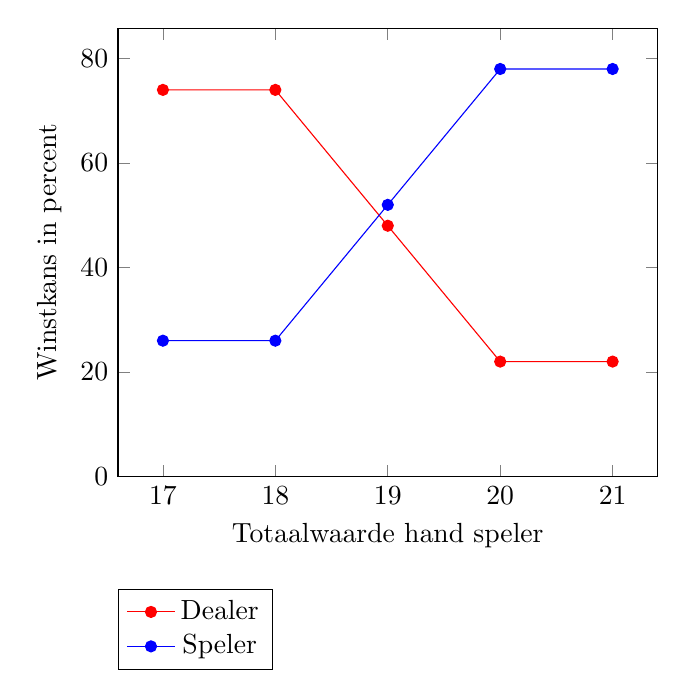
\begin{tikzpicture}
    \begin{axis}[xlabel=Totaalwaarde hand speler,
								ylabel=Winstkans in percent,
								legend style={
								at={(0,0)},
								anchor=north west,at={(axis description cs:0,-0.25)}}, 
								ymin=0]
    \addplot[mark=*, color=red] coordinates{
				(17,74)
				(18,74)
				(19,48)
				(20,22)
				(21,22)
		};
		\addlegendentry{Dealer}
		\addplot[mark=*, color=blue] coordinates{
				(17,26)
				(18,26)
				(19,52)
				(20,78)
				(21,78)
		};
		\addlegendentry{Speler}
    \end{axis}
		\end{tikzpicture}
}\\
\caption{Grafiek die de winstkans van de speler tegenover de deler weergeeft bij verschillende totaalwaardes van de hand.}%
\end{center}
\end{figure}
\\
\subsection{Resultaten splitten}
Om deze resultaten te bekomen hebben we elk hand 10000 keer gesimuleerd. Vervolgens keken we wie de winnaar is. Om dit te bekomen, hebben we ervoor gezorgd dat de speler telkens twee dezelfde kaarten in zijn hand heeft. De speler zal de ene keer de kaarten splitten, terwijl hij de volgende keer met hetzelfde hand niet zal splitsen.
Volgende resultaten werden bekomen:\\
\begin{table}[h]
\begin{tabular}{c||c|c||c||c|c||c|}
\multicolumn{1}{l||}{}       							& \multicolumn{6}{c|}{Speler gesplit}                            \\ \cline{2-7} 
																					& \multicolumn{3}{c||}{Ja}      & \multicolumn{3}{c|}{Nee}       \\ \cline{2-7} 
																					& \multicolumn{3}{c||}{Winnaar} & \multicolumn{3}{c|}{Winnaar}   \\ \hline 
\multicolumn{1}{c||}{Speler hand}					& Dealer  & Speler   & Totaal  	& Dealer    & Speler  & Totaal   \\ \hline
\multicolumn{1}{r||}{2-2}   							& 32\%    & 68\%     & 100\%   	& 60\%     	& 40\%    & 100\%    \\ \hline
\multicolumn{1}{r||}{3-3}   							& 34\%    & 66\%     & 100\%   	& 61\%     	& 39\%    & 100\%    \\ \hline
\multicolumn{1}{r||}{4-4}   							& 45\%    & 55\%     & 100\%   	& 71\%     	& 29\%    & 100\%    \\ \hline
\multicolumn{1}{r||}{5-5}   							& 42\%    & 58\%     & 100\%   	& 55\%     	& 45\%    & 100\%    \\ \hline
\multicolumn{1}{r||}{6-6}   							& 43\%    & 57\%     & 100\%   	& 68\%     	& 32\%    & 100\%    \\ \hline
\multicolumn{1}{r||}{7-7}   							& 44\%    & 56\%     & 100\%   	& 61\%     	& 39\%    & 100\%    \\ \hline
\multicolumn{1}{r||}{8-8}   							& 36\%    & 64\%     & 100\%   	& 30\%     	& 70\%    & 100\%    \\ \hline
\multicolumn{1}{r||}{9-9}   							& 26\%    & 74\%     & 100\%   	& 39\%     	& 61\%    & 100\%    \\ \hline
\multicolumn{1}{r||}{10-10} 							& 18\%    & 82\%     & 100\%   	& 8\%      	& 92\%    & 100\%    \\ \hline
\multicolumn{1}{r||}{A-A}   							& 10\%    & 90\%     & 100\%   	& 8\%      	& 92\%    & 100\%    \\	\hline \hline
\multicolumn{1}{r||}{Gemiddelde}					& 33\%		& 67\%		 & 100\%   	& 46\%			& 54\%		& 100\%		 \\
\end{tabular}
\end{table}
\\

Deze gegevens zijn ook hier representatief in een bijhorende lijndiagram. De assen voor de dealer zijn verwijderd omdat deze het complement zijn van de speler, tevens zou dit de diagram te complex en moeilijk om lezen maken.

\begin{figure}[h]%
\begin{center}
\subfigure{
    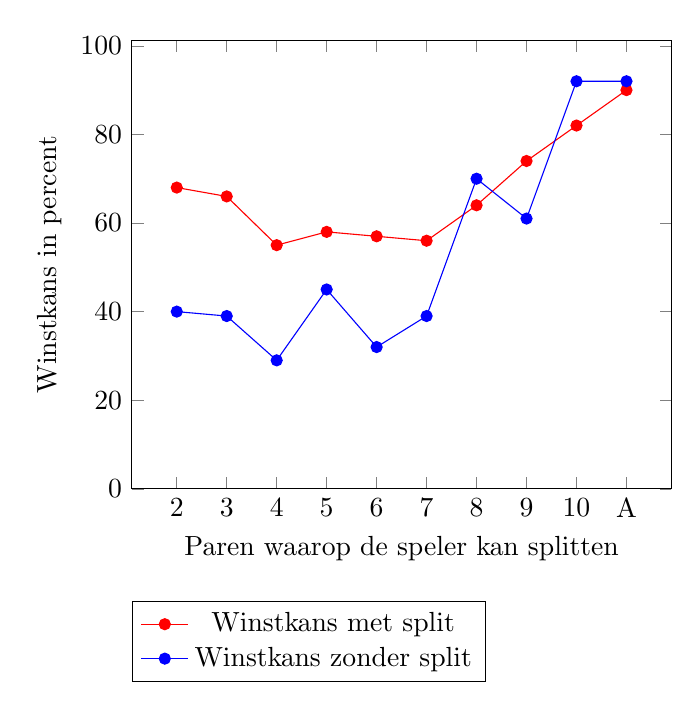
\begin{tikzpicture}
    \begin{axis}[xlabel=Paren waarop de speler kan splitten,
								ylabel=Winstkans in percent,
								legend style={
								at={(0,0)},
								anchor=north west,at={(axis description cs:0,-0.25)}}, 
								ymin=0, 
								xtick=data, 
								xticklabels={2,3,4,5,6,7,8,9,10,A}]
		\addplot[mark=*, color=red] coordinates{
				(1,68)
				(2,66)
				(3,55)
				(4,58)
				(5,57)
				(6,56)
				(7,64)
				(8,74)
				(9,82)
				(10,90)
		};
		\addlegendentry{Winstkans met split}
		\addplot[mark=*, color=blue] coordinates{
				(1,40)
				(2,39)
				(3,29)
				(4,45)
				(5,32)
				(6,39)
				(7,70)
				(8,61)
				(9,92)
				(10,92)
		};
		\addlegendentry{Winstkans zonder split}
    \end{axis}
		\end{tikzpicture}
}\\
\caption{Grafiek die de winstkans van de speler weergeeft bij splitten en niet splitten op specifieke paren.}%
\end{center}
\end{figure}

\section{Discussie/bespreking}
In dit onderzoek gingen we na welke waarde het meest ideaal is om te standen en te splitten. Hiervoor hebben we gebruik gemaakt van onze aangepaste simulatiesoftware. Uit de resultaten van de berekeningen betreffende standen leiden we af dat de speler voor een totaalwaarde kleiner dan 19 slechts 26\% kans heeft om de dealer te verslaan. Het is logisch dat een speler onder een totaalwaarde van 17 weinig kans heeft om te winnen, aangezien de dealer blijft hitten tot 17 en in de meeste gevallen boven de speler zal uit komen. De momenten dat de speler wel kan winnen, zijn wanneer de dealer zich burnt en de speler dus automatisch de winnaar is. Dit komt neer op de 26\% die we gevonden hebben.

Bij de totaalwaarden groter dan 18 is het snel duidelijk dat de speler de bovenhand krijgt en met 52\% en meer wint naarmate de totaalwaarde groter wordt. Dit is een logische uitkomst aangezien de dealer moeilijk boven de speler geraakt zonder zichzelf te burnen. Toch moeten we hierbij een aantal zaken opmerken. In deze simulatie heeft de speler een vaste totaalwaarde, maar in een realistische situatie zal het veel moeilijker zijn om aan deze hoge waarden te geraken. Dit wil dus zeggen dat, ook al heeft de speler in de simulatie veel meer kans om te winnen, de kans dat de speler zo’n totaalwaarde krijgt tijdens een spel heel wat lager zal liggen, waardoor de dealer opnieuw een voordeel heeft. Als we een gemiddelde nemen van alle percentages, valt het ons op dat de dealer sowieso de bovenhand heeft met 67,5\% tegenover de speler met 32,5\%. In het algemeen heeft de speler dus minder kans om te winnen. Toch moeten we rekening houden met de beperkingen die reeds in het vorige onderdeel werden besproken.

Als laatste willen we graag opmerken dat de dealer toch nog 26\% winst behaalt als de speler een totaalwaarde van 21 heeft. Dit telt dan als een push en geldt dan als een win voor de dealer.

Tot slot de berekeningen over het ideaal splitcijfer. De tabel toont per hand vier procenten. Het ja gedeelte betekent dat de speler split bij twee gelijke kaarten, in het nee gedeelte geven we de cijfers weer indien de speler niet split. Het percent zelf omvat het aantal keer winst. De twee percenten onder ja en nee vormen dus samen 100\%. 

Het winstpercentage van de speler ligt over het algemeen zeer hoog. Als eerste zullen we de ja-tabel bekijken. Hier wint de speler altijd meer dan 50\%. Dit komt simpelweg omdat u bij het splitten twee hands hebt. In onze simulator houden we enkel rekening met het winnende hand. Hand a kan dus geburnt zijn terwijl hand b de dealer verslaat met een 20. Aan de nee zijde zien we dat de procenten vanaf acht zeer snel stijgen. In een spel met onze parameters is het dus beter om te splitten tot en met zeven. De winstcijfers van de hogere kaarten liggen dichter bij elkaar. Zo ziet u dat bij twee azen de winstkans met maar twee procent verschilt. Tot slot merken we toch wel op dat de algemene winstkans voor de speler hoger ligt indien men split. 

\section{Besluit}
In dit artikel hebben we onderzoek gedaan naar de totaalwaarde om te standen en wanneer men het beste kan splitten. Uit de resultaten van ons onderzoek kunnen we afleiden dat een speler het best stand als hij een hand hoger dan 18 heeft, maar dat de kans dan bestaat dat de speler geburnt is vooraleer hij hieraan geraakt. Uit de gemiddelde resultaten blijkt dat de dealer voor 67,5\% een voorsprong heeft.

Als we naar de resultaten van het splitten kijken, merken we dat de gemiddelde winstkans voor de speler meer dan 10\% hoger ligt indien hij split dan als hij niet split. Over het algemeen kunnen we dus stellen dat de speler best split vanaf hij de kans heeft, maar bij sommige gevallen heeft de speler toch meer winstkans indien hij niet split. Dit is het geval bij de paren 8-8 waar hij 6\% meer kans heeft om te winnen indien hij niet split, A-A waar hij slechts 2\% kans meer heeft om te winnen en 10-10, hier heeft de speler een groot voordeel van 10\% indien hij niet beslist te splitten.

\bibliographystyle{apa}

\bibliography{Blackjack}

\end{document}